\begin{frame}{Design process - \Romannum{1}}
    \only<1>{
        \begin{figure}
            \centering
            \newcommand\WIDTH{3cm}
\newcommand\HEIGHT{1.25cm}
\newcommand\Ydist{0.2cm}
\newcommand\XPOS{2cm}
\newcommand\TOTheight{6.2cm}
\newcommand\TOTwidth{3.4cm}
\newcommand\PTS{1.2pt}
\newcommand\SHADOWred{50}
\newcommand\SHADOWgreen{30}
\newcommand\SHADOWblue{20}

\begin{tikzpicture}
    
    \node[draw,
        rectangle,
        % rounded corners,
        line width = \PTS,
        minimum height = \TOTheight,
        minimum width = \TOTwidth
    ] (man) at (0, 0) {};

    \node[draw,
        rectangle,
        % rounded corners,
        line width = \PTS,
        minimum height = \TOTheight,
        minimum width = \TOTwidth,
        right = \XPOS of man
    ] (auto) {};

    % \node[draw,
    %     rectangle,
    %     % rounded corners,
    %     line width = \PTS,
    %     minimum height = \TOTheight,
    %     minimum width = \TOTwidth,
    %     right = \XPOS of auto
    % ] (ml) {};

    \node[draw, 
        rectangle,
        fill = blue!\SHADOWblue,
        line width = \PTS,
        minimum height = 0.8cm,
        above right = -\PTS and 0cm of man.north west
    ] (manTitle) {\textbf{\large{Manual}}};

    \node[draw, 
        rectangle,
        fill = blue!\SHADOWblue,
        line width = \PTS,
        minimum height = 0.8cm,
        above right = -\PTS and 0cm of auto.north west
    ] (autoTitle) {\textbf{\large{Automated}}};

    % \node[draw, 
    %     rectangle,
    %     fill = blue!\SHADOWblue,
    %     line width = \PTS,
    %     minimum height = 1.5cm,
    %     above right = -\PTS and 0cm of ml.north west
    % ] (mlTitle) {\textbf{\Huge{Machine learning}}};

    \node[draw,
        rectangle,
        rounded corners,
        line width = \PTS,
        minimum width = \WIDTH,
        minimum height = \HEIGHT, 
        % fill = red!\SHADOWred,
        below = \Ydist of man.north
    ] (manCFD) {\textbf{\small{Iterative CFD}}};

    \node[draw,
        rectangle,
        rounded corners,
        line width = \PTS,
        minimum width = \WIDTH,
        minimum height = \HEIGHT,
        below = \Ydist of manCFD
    ] (manObj) {\makecell[c]{\textbf{\small{Objectives \&}} \\ \textbf{\small{constraints}}}};%{\textbf{\Large{Objectives \& constraints}}};

    \node[draw,
        rectangle,
        rounded corners,
        line width = \PTS,
        minimum width = \WIDTH,
        minimum height = \HEIGHT,
        below = \Ydist of manObj,
        % fill = green!\SHADOWgreen
    ] (manKnow) {\makecell[c]{\textbf{\small{Using prior}} \\ \textbf{\small{knowledge}}}}; %{\textbf{Using prior knowledge}};

    \node[draw,
        rectangle,
        rounded corners,
        line width = \PTS,
        minimum width = \WIDTH,
        minimum height = \HEIGHT,
        below = \Ydist of manKnow,
        % fill = red!\SHADOWred
    ] (manMan) {\textbf{\small{Manual}}};

    \node[draw,
        rectangle,
        rounded corners,
        line width = \PTS,
        minimum width = \WIDTH,
        minimum height = \HEIGHT, 
        below = \Ydist of auto.north,
        % fill = red!\SHADOWred
    ] (autoCFD) {\textbf{\small{Iterative CFD}}};

    \node[draw,
        rectangle,
        rounded corners,
        line width = \PTS,
        minimum width = \WIDTH,
        minimum height = \HEIGHT,
        below = \Ydist of autoCFD
    ] (autoObj) {\makecell[c]{\textbf{\small{Objectives \&}} \\ \textbf{\small{constraints}}}};%{\textbf{\Large{Objectives \& constraints}}};

    \node[draw,
        rectangle,
        rounded corners,
        line width = \PTS,
        minimum width = \WIDTH,
        minimum height = \HEIGHT,
        below = \Ydist of autoObj,
        % fill = red!\SHADOWred
    ] (autoKnow) {\makecell[c]{\textbf{\small{Not using prior}} \\ \textbf{\small{knowledge}}}};

    \node[draw,
        rectangle,
        rounded corners,
        line width = \PTS,
        minimum width = \WIDTH,
        minimum height = \HEIGHT,
        below = \Ydist of autoKnow,
        % fill = green!\SHADOWgreen
    ] (autoAuto) {\textbf{\small{Automated}}}; 

    % \node[draw,
    %     rectangle,
    %     rounded corners,
    %     line width = \PTS,
    %     minimum width = \WIDTH
    %     minimum height = \HEIGHT, 
    %     below = \Ydist of ml.north,
    %     fill = green!\SHADOWgreen
    % ] (mlCFD) {\textbf{\Large{Regression}}};

    % \node[draw,
    %     rectangle,
    %     rounded corners,
    %     line width = \PTS,
    %     minimum width = \WIDTH,
    %     minimum height = \HEIGHT,
    %     below = \Ydist of mlCFD,
    %     fill = green!\SHADOWgreen
    % ] (mlObj) {\makecell[c]{\textbf{\Large{Aerodynamic duty \&}} \\ \textbf{\Large{aerodynamic style}}}};%{\textbf{\Large{Objectives \& constraints}}};

    % \node[draw,
    %     rectangle,
    %     rounded corners,
    %     line width = \PTS,
    %     minimum width = \WIDTH,
    %     minimum height = \HEIGHT,
    %     below = \Ydist of mlObj,
    %     fill = green!\SHADOWgreen
    % ] (mlKnow) {\makecell[c]{\textbf{\Large{Using prior}} \\ \textbf{\Large{knowledge}}}};

    % \node[draw,
    %     rectangle,
    %     rounded corners,
    %     line width = \PTS,
    %     minimum width = \WIDTH,
    %     minimum height = \HEIGHT,
    %     below = \Ydist of mlKnow,
    %     fill = green!\SHADOWgreen
    % ] (mlAuto) {\textbf{\Large{Automated}}}; 
 
\end{tikzpicture}

            % 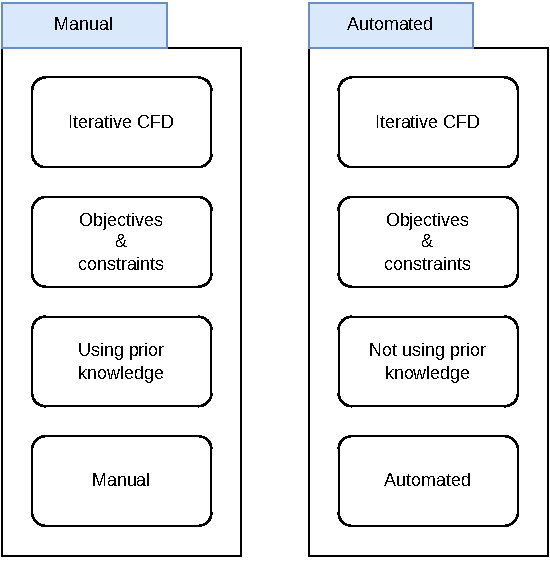
\includegraphics[page=1, scale=0.75]{pdf/designModes-00}
        \end{figure}
    }
    \only<2>{
        \begin{figure}
            \centering
            \newcommand\WIDTH{3cm}
\newcommand\HEIGHT{1.25cm}
\newcommand\Ydist{0.2cm}
\newcommand\XPOS{2cm}
\newcommand\TOTheight{6.2cm}
\newcommand\TOTwidth{3.4cm}
\newcommand\PTS{1.2pt}
\newcommand\SHADOWred{50}
\newcommand\SHADOWgreen{30}
\newcommand\SHADOWblue{20}

\begin{tikzpicture}
    
    \node[draw,
        rectangle,
        % rounded corners,
        line width = \PTS,
        minimum height = \TOTheight,
        minimum width = \TOTwidth
    ] (man) at (0, 0) {};

    \node[draw,
        rectangle,
        % rounded corners,
        line width = \PTS,
        minimum height = \TOTheight,
        minimum width = \TOTwidth,
        right = \XPOS of man
    ] (auto) {};

    % \node[draw,
    %     rectangle,
    %     % rounded corners,
    %     line width = \PTS,
    %     minimum height = \TOTheight,
    %     minimum width = \TOTwidth,
    %     right = \XPOS of auto
    % ] (ml) {};

    \node[draw, 
        rectangle,
        fill = blue!\SHADOWblue,
        line width = \PTS,
        minimum height = 0.8cm,
        above right = -\PTS and 0cm of man.north west
    ] (manTitle) {\textbf{\large{Manual}}};

    \node[draw, 
        rectangle,
        fill = blue!\SHADOWblue,
        line width = \PTS,
        minimum height = 0.8cm,
        above right = -\PTS and 0cm of auto.north west
    ] (autoTitle) {\textbf{\large{Automated}}};

    % \node[draw, 
    %     rectangle,
    %     fill = blue!\SHADOWblue,
    %     line width = \PTS,
    %     minimum height = 1.5cm,
    %     above right = -\PTS and 0cm of ml.north west
    % ] (mlTitle) {\textbf{\Huge{Machine learning}}};

    \node[draw,
        rectangle,
        rounded corners,
        line width = \PTS,
        minimum width = \WIDTH,
        minimum height = \HEIGHT, 
        fill = red!\SHADOWred,
        below = \Ydist of man.north
    ] (manCFD) {\textbf{\small{Iterative CFD}}};

    \node[draw,
        rectangle,
        rounded corners,
        line width = \PTS,
        minimum width = \WIDTH,
        minimum height = \HEIGHT,
        below = \Ydist of manCFD
    ] (manObj) {\makecell[c]{\textbf{\small{Objectives \&}} \\ \textbf{\small{constraints}}}};%{\textbf{\Large{Objectives \& constraints}}};

    \node[draw,
        rectangle,
        rounded corners,
        line width = \PTS,
        minimum width = \WIDTH,
        minimum height = \HEIGHT,
        below = \Ydist of manObj,
        fill = green!\SHADOWgreen
    ] (manKnow) {\makecell[c]{\textbf{\small{Using prior}} \\ \textbf{\small{knowledge}}}}; %{\textbf{Using prior knowledge}};

    \node[draw,
        rectangle,
        rounded corners,
        line width = \PTS,
        minimum width = \WIDTH,
        minimum height = \HEIGHT,
        below = \Ydist of manKnow,
        fill = red!\SHADOWred
    ] (manMan) {\textbf{\small{Manual}}};

    \node[draw,
        rectangle,
        rounded corners,
        line width = \PTS,
        minimum width = \WIDTH,
        minimum height = \HEIGHT, 
        below = \Ydist of auto.north,
        fill = red!\SHADOWred
    ] (autoCFD) {\textbf{\small{Iterative CFD}}};

    \node[draw,
        rectangle,
        rounded corners,
        line width = \PTS,
        minimum width = \WIDTH,
        minimum height = \HEIGHT,
        below = \Ydist of autoCFD
    ] (autoObj) {\makecell[c]{\textbf{\small{Objectives \&}} \\ \textbf{\small{constraints}}}};%{\textbf{\Large{Objectives \& constraints}}};

    \node[draw,
        rectangle,
        rounded corners,
        line width = \PTS,
        minimum width = \WIDTH,
        minimum height = \HEIGHT,
        below = \Ydist of autoObj,
        fill = red!\SHADOWred
    ] (autoKnow) {\makecell[c]{\textbf{\small{Not using prior}} \\ \textbf{\small{knowledge}}}};

    \node[draw,
        rectangle,
        rounded corners,
        line width = \PTS,
        minimum width = \WIDTH,
        minimum height = \HEIGHT,
        below = \Ydist of autoKnow,
        fill = green!\SHADOWgreen
    ] (autoAuto) {\textbf{\small{Automated}}}; 

    % \node[draw,
    %     rectangle,
    %     rounded corners,
    %     line width = \PTS,
    %     minimum width = \WIDTH
    %     minimum height = \HEIGHT, 
    %     below = \Ydist of ml.north,
    %     fill = green!\SHADOWgreen
    % ] (mlCFD) {\textbf{\Large{Regression}}};

    % \node[draw,
    %     rectangle,
    %     rounded corners,
    %     line width = \PTS,
    %     minimum width = \WIDTH,
    %     minimum height = \HEIGHT,
    %     below = \Ydist of mlCFD,
    %     fill = green!\SHADOWgreen
    % ] (mlObj) {\makecell[c]{\textbf{\Large{Aerodynamic duty \&}} \\ \textbf{\Large{aerodynamic style}}}};%{\textbf{\Large{Objectives \& constraints}}};

    % \node[draw,
    %     rectangle,
    %     rounded corners,
    %     line width = \PTS,
    %     minimum width = \WIDTH,
    %     minimum height = \HEIGHT,
    %     below = \Ydist of mlObj,
    %     fill = green!\SHADOWgreen
    % ] (mlKnow) {\makecell[c]{\textbf{\Large{Using prior}} \\ \textbf{\Large{knowledge}}}};

    % \node[draw,
    %     rectangle,
    %     rounded corners,
    %     line width = \PTS,
    %     minimum width = \WIDTH,
    %     minimum height = \HEIGHT,
    %     below = \Ydist of mlKnow,
    %     fill = green!\SHADOWgreen
    % ] (mlAuto) {\textbf{\Large{Automated}}}; 
 
\end{tikzpicture}

            % 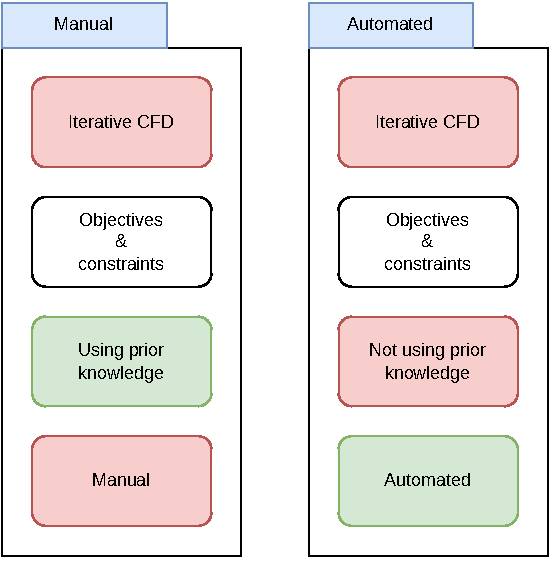
\includegraphics[page=1, scale=0.75]{pdf/designModes-01}
        \end{figure}
    }
    \only<3>{
        \begin{figure}
            \centering
            \newcommand\WIDTH{3cm}
\newcommand\HEIGHT{1.25cm}
\newcommand\Ydist{0.2cm}
\newcommand\XPOS{2cm}
\newcommand\TOTheight{6.2cm}
\newcommand\TOTwidth{3.4cm}
\newcommand\PTS{1.2pt}
\newcommand\SHADOWred{50}
\newcommand\SHADOWgreen{30}
\newcommand\SHADOWblue{20}

\vspace{-0.5cm}

\begin{tikzpicture}
    
    \node[draw,
        rectangle,
        % rounded corners,
        line width = \PTS,
        minimum height = \TOTheight,
        minimum width = \TOTwidth
    ] (man) at (0, 0) {};

    \node[draw,
        rectangle,
        % rounded corners,
        line width = \PTS,
        minimum height = \TOTheight,
        minimum width = \TOTwidth,
        right = \XPOS of man
    ] (auto) {};

    \node[draw,
        rectangle,
        % rounded corners,
        line width = \PTS,
        minimum height = \TOTheight,
        minimum width = \TOTwidth,
        right = \XPOS of auto
    ] (ml) {};

    \node[draw, 
        rectangle,
        fill = blue!\SHADOWblue,
        line width = \PTS,
        minimum height = 0.8cm,
        above right = -\PTS and 0cm of man.north west
    ] (manTitle) {\textbf{\small{Manual}}};

    \node[draw, 
        rectangle,
        fill = blue!\SHADOWblue,
        line width = \PTS,
        minimum height = 0.8cm,
        above right = -\PTS and 0cm of auto.north west
    ] (autoTitle) {\textbf{\small{Automated}}};

    \node[draw, 
        rectangle,
        fill = blue!\SHADOWblue,
        line width = \PTS,
        minimum height = 0.8cm,
        above right = -\PTS and 0cm of ml.north west
    ] (mlTitle) {\textbf{\small{Machine learning}}};

    \node[draw,
        rectangle,
        rounded corners,
        line width = \PTS,
        minimum width = \WIDTH,
        minimum height = \HEIGHT, 
        % fill = red!\SHADOWred,
        below = \Ydist of man.north
    ] (manCFD) {\textbf{\small{Iterative CFD}}};

    \node[draw,
        rectangle,
        rounded corners,
        line width = \PTS,
        minimum width = \WIDTH,
        minimum height = \HEIGHT,
        below = \Ydist of manCFD
    ] (manObj) {\makecell[c]{\textbf{\small{Objectives \&}} \\ \textbf{\small{constraints}}}};%{\textbf{\small{Objectives \& constraints}}};

    \node[draw,
        rectangle,
        rounded corners,
        line width = \PTS,
        minimum width = \WIDTH,
        minimum height = \HEIGHT,
        below = \Ydist of manObj,
        fill = green!\SHADOWgreen
    ] (manKnow) {\makecell[c]{\textbf{\small{Using prior}} \\ \textbf{\small{knowledge}}}}; %{\textbf{Using prior knowledge}};

    \node[draw,
        rectangle,
        rounded corners,
        line width = \PTS,
        minimum width = \WIDTH,
        minimum height = \HEIGHT,
        below = \Ydist of manKnow,
        % fill = red!\SHADOWred
    ] (manMan) {\textbf{\small{Manual}}};

    \node[draw,
        rectangle,
        rounded corners,
        line width = \PTS,
        minimum width = \WIDTH,
        minimum height = \HEIGHT, 
        below = \Ydist of auto.north,
        % fill = red!\SHADOWred
    ] (autoCFD) {\textbf{\small{Iterative CFD}}};

    \node[draw,
        rectangle,
        rounded corners,
        line width = \PTS,
        minimum width = \WIDTH,
        minimum height = \HEIGHT,
        below = \Ydist of autoCFD
    ] (autoObj) {\makecell[c]{\textbf{\small{Objectives \&}} \\ \textbf{\small{constraints}}}};%{\textbf{\small{Objectives \& constraints}}};

    \node[draw,
        rectangle,
        rounded corners,
        line width = \PTS,
        minimum width = \WIDTH,
        minimum height = \HEIGHT,
        below = \Ydist of autoObj,
        % fill = red!\SHADOWred
    ] (autoKnow) {\makecell[c]{\textbf{\small{Not using prior}} \\ \textbf{\small{knowledge}}}};

    \node[draw,
        rectangle,
        rounded corners,
        line width = \PTS,
        minimum width = \WIDTH,
        minimum height = \HEIGHT,
        below = \Ydist of autoKnow,
        fill = green!\SHADOWgreen
    ] (autoAuto) {\textbf{\small{Automated}}}; 

    \node[draw,
        rectangle,
        rounded corners,
        line width = \PTS,
        minimum width = \WIDTH,
        minimum height = \HEIGHT, 
        below = \Ydist of ml.north,
        % fill = green!\SHADOWgreen
    ] (mlCFD) {};%{\textbf{\small{Regression}}};

    \node[draw,
        rectangle,
        rounded corners,
        line width = \PTS,
        minimum width = \WIDTH,
        minimum height = \HEIGHT,
        below = \Ydist of mlCFD,
        % fill = green!\SHADOWgreen
    ] (mlObj) {};%{\makecell[c]{\textbf{\small{Aerodynamic duty \&}} \\ \textbf{\small{aerodynamic style}}}};%{\textbf{\small{Objectives \& constraints}}};

    \node[draw,
        rectangle,
        rounded corners,
        line width = \PTS,
        minimum width = \WIDTH,
        minimum height = \HEIGHT,
        below = \Ydist of mlObj,
        fill = green!\SHADOWgreen
    ] (mlKnow) {\makecell[c]{\textbf{\small{Using prior}} \\ \textbf{\small{knowledge}}}};

    \node[draw,
        rectangle,
        rounded corners,
        line width = \PTS,
        minimum width = \WIDTH,
        minimum height = \HEIGHT,
        below = \Ydist of mlKnow,
        fill = green!\SHADOWgreen
    ] (mlAuto) {\textbf{\small{Automated}}}; 
 
\end{tikzpicture}

            % 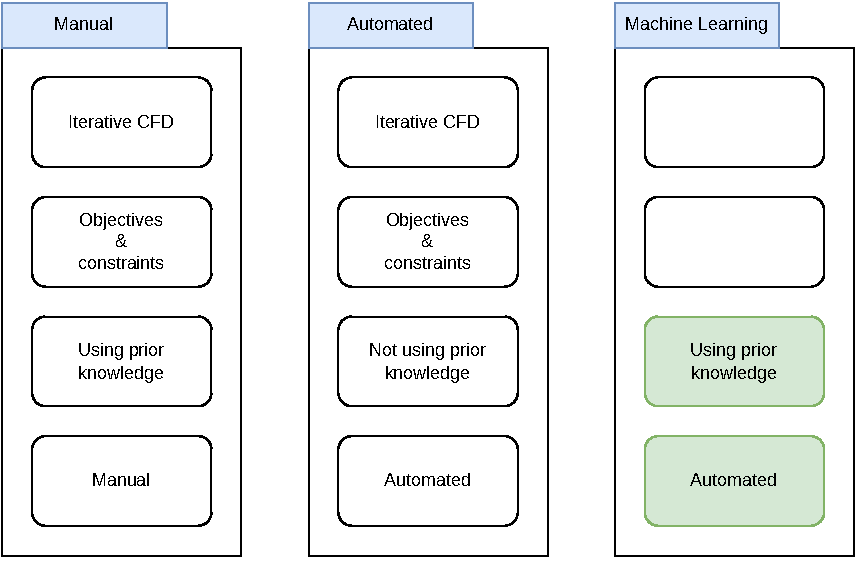
\includegraphics[page=1, scale=0.75]{pdf/designModes-02}
        \end{figure}
    }
\end{frame}

\begin{frame}{Data in turbomachinery design}
    \vspace{0.5cm}
    These points allow to use a \textbf{regression based model} to design a blade.
    \vspace{0.5cm}
    \begin{itemize}
        \setlength{\itemsep}{15pt}
        \item Turbomachinery design physics \textbf{is not stochastic}
        \item Turbomachinery design is \textbf{multi-objectives} and \textbf{multi-constrained}
        \item Turbomachinery blades are \textbf{high dimensional objects}
    \end{itemize}
    \vspace{0.5cm}
    The blade has to be parametrized by \textbf{few parameters} after a \textbf{design space reduction}. \\
    
    \vspace{0.5cm}
    Data collection has to \textbf{correlate} the \textbf{design objectives} to the \textbf{blade geometry}.
\end{frame}

\begin{frame}{Design process - \Romannum{2}}
    \begin{figure}
        \centering
        \newcommand\WIDTH{3cm}
\newcommand\HEIGHT{1.25cm}
\newcommand\Ydist{0.2cm}
\newcommand\XPOS{2cm}
\newcommand\TOTheight{6.2cm}
\newcommand\TOTwidth{3.4cm}
\newcommand\PTS{1.2pt}
\newcommand\SHADOWred{50}
\newcommand\SHADOWgreen{30}
\newcommand\SHADOWblue{20}

\vspace{-0.5cm}

\begin{tikzpicture}
    
    \node[draw,
        rectangle,
        % rounded corners,
        line width = \PTS,
        minimum height = \TOTheight,
        minimum width = \TOTwidth
    ] (man) at (0, 0) {};

    \node[draw,
        rectangle,
        % rounded corners,
        line width = \PTS,
        minimum height = \TOTheight,
        minimum width = \TOTwidth,
        right = \XPOS of man
    ] (auto) {};

    \node[draw,
        rectangle,
        % rounded corners,
        line width = \PTS,
        minimum height = \TOTheight,
        minimum width = \TOTwidth,
        right = \XPOS of auto
    ] (ml) {};

    \node[draw, 
        rectangle,
        fill = blue!\SHADOWblue,
        line width = \PTS,
        minimum height = 0.8cm,
        above right = -\PTS and 0cm of man.north west
    ] (manTitle) {\textbf{\small{Manual}}};

    \node[draw, 
        rectangle,
        fill = blue!\SHADOWblue,
        line width = \PTS,
        minimum height = 0.8cm,
        above right = -\PTS and 0cm of auto.north west
    ] (autoTitle) {\textbf{\small{Automated}}};

    \node[draw, 
        rectangle,
        fill = blue!\SHADOWblue,
        line width = \PTS,
        minimum height = 0.8cm,
        above right = -\PTS and 0cm of ml.north west
    ] (mlTitle) {\textbf{\small{Machine learning}}};

    \node[draw,
        rectangle,
        rounded corners,
        line width = \PTS,
        minimum width = \WIDTH,
        minimum height = \HEIGHT, 
        % fill = red!\SHADOWred,
        below = \Ydist of man.north
    ] (manCFD) {\textbf{\small{Iterative CFD}}};

    \node[draw,
        rectangle,
        rounded corners,
        line width = \PTS,
        minimum width = \WIDTH,
        minimum height = \HEIGHT,
        below = \Ydist of manCFD
    ] (manObj) {\makecell[c]{\textbf{\small{Objectives \&}} \\ \textbf{\small{constraints}}}};%{\textbf{\small{Objectives \& constraints}}};

    \node[draw,
        rectangle,
        rounded corners,
        line width = \PTS,
        minimum width = \WIDTH,
        minimum height = \HEIGHT,
        below = \Ydist of manObj,
        fill = green!\SHADOWgreen
    ] (manKnow) {\makecell[c]{\textbf{\small{Using prior}} \\ \textbf{\small{knowledge}}}}; %{\textbf{Using prior knowledge}};

    \node[draw,
        rectangle,
        rounded corners,
        line width = \PTS,
        minimum width = \WIDTH,
        minimum height = \HEIGHT,
        below = \Ydist of manKnow,
        % fill = red!\SHADOWred
    ] (manMan) {\textbf{\small{Manual}}};

    \node[draw,
        rectangle,
        rounded corners,
        line width = \PTS,
        minimum width = \WIDTH,
        minimum height = \HEIGHT, 
        below = \Ydist of auto.north,
        % fill = red!\SHADOWred
    ] (autoCFD) {\textbf{\small{Iterative CFD}}};

    \node[draw,
        rectangle,
        rounded corners,
        line width = \PTS,
        minimum width = \WIDTH,
        minimum height = \HEIGHT,
        below = \Ydist of autoCFD
    ] (autoObj) {\makecell[c]{\textbf{\small{Objectives \&}} \\ \textbf{\small{constraints}}}};%{\textbf{\small{Objectives \& constraints}}};

    \node[draw,
        rectangle,
        rounded corners,
        line width = \PTS,
        minimum width = \WIDTH,
        minimum height = \HEIGHT,
        below = \Ydist of autoObj,
        % fill = red!\SHADOWred
    ] (autoKnow) {\makecell[c]{\textbf{\small{Not using prior}} \\ \textbf{\small{knowledge}}}};

    \node[draw,
        rectangle,
        rounded corners,
        line width = \PTS,
        minimum width = \WIDTH,
        minimum height = \HEIGHT,
        below = \Ydist of autoKnow,
        fill = green!\SHADOWgreen
    ] (autoAuto) {\textbf{\small{Automated}}}; 

    \node[draw,
        rectangle,
        rounded corners,
        line width = \PTS,
        minimum width = \WIDTH,
        minimum height = \HEIGHT, 
        below = \Ydist of ml.north,
        fill = green!\SHADOWgreen
    ] (mlCFD) {\textbf{\small{Regression}}};

    \node[draw,
        rectangle,
        rounded corners,
        line width = \PTS,
        minimum width = \WIDTH,
        minimum height = \HEIGHT,
        below = \Ydist of mlCFD,
        % fill = green!\SHADOWgreen
    ] (mlObj) {};%{\makecell[c]{\textbf{\small{Aerodynamic duty \&}} \\ \textbf{\small{aerodynamic style}}}};%{\textbf{\small{Objectives \& constraints}}};

    \node[draw,
        rectangle,
        rounded corners,
        line width = \PTS,
        minimum width = \WIDTH,
        minimum height = \HEIGHT,
        below = \Ydist of mlObj,
        fill = green!\SHADOWgreen
    ] (mlKnow) {\makecell[c]{\textbf{\small{Using prior}} \\ \textbf{\small{knowledge}}}};

    \node[draw,
        rectangle,
        rounded corners,
        line width = \PTS,
        minimum width = \WIDTH,
        minimum height = \HEIGHT,
        below = \Ydist of mlKnow,
        fill = green!\SHADOWgreen
    ] (mlAuto) {\textbf{\small{Automated}}}; 
 
\end{tikzpicture}

        % 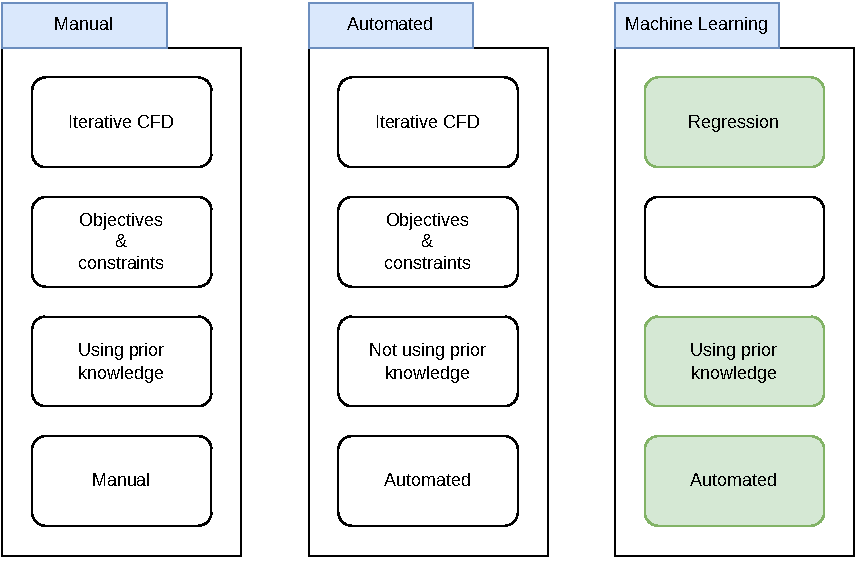
\includegraphics[page=1, scale=0.75]{pdf/designModes-03}
    \end{figure}
\end{frame}

\begin{frame}{Data features}
    \vspace{0.5cm}
    % The design tool \textbf{does not have objectives neither constraints}. 
    % \newline
    % \vspace{0.2cm}
    
    The computed data has to \textbf{map} the objective domain satisfying the constraints. 
    \newline
    \vspace{0.2cm}
    
    This can be achieved using appropriate \textbf{design features}.
    \newline
    \vspace{0.2cm}
    
    In order to collect all these information, the data will depend on two new \textbf{aerodynamic features}: 
    \newline
    \vspace{0.2cm}

    \begin{itemize}
        \setlength{\itemsep}{15pt}
        \item \textbf{Aerodynamic duty}: a domain of study that allows \textbf{mapping} the constraints
        \item \textbf{Aerodynamic style}: a domain of study that allows \textbf{mapping} the objectives
    \end{itemize} 
\end{frame}

\begin{frame}{Design process - \Romannum{3}}
    \begin{figure}
        \centering
        \newcommand\WIDTH{3cm}
\newcommand\HEIGHT{1.25cm}
\newcommand\Ydist{0.2cm}
\newcommand\XPOS{2cm}
\newcommand\TOTheight{6.2cm}
\newcommand\TOTwidth{3.4cm}
\newcommand\PTS{1.2pt}
\newcommand\SHADOWred{50}
\newcommand\SHADOWgreen{30}
\newcommand\SHADOWblue{20}

\vspace{-0.5cm}

\begin{tikzpicture}
    
    \node[draw,
        rectangle,
        % rounded corners,
        line width = \PTS,
        minimum height = \TOTheight,
        minimum width = \TOTwidth
    ] (man) at (0, 0) {};

    \node[draw,
        rectangle,
        % rounded corners,
        line width = \PTS,
        minimum height = \TOTheight,
        minimum width = \TOTwidth,
        right = \XPOS of man
    ] (auto) {};

    \node[draw,
        rectangle,
        % rounded corners,
        line width = \PTS,
        minimum height = \TOTheight,
        minimum width = \TOTwidth,
        right = \XPOS of auto
    ] (ml) {};

    \node[draw, 
        rectangle,
        fill = blue!\SHADOWblue,
        line width = \PTS,
        minimum height = 0.8cm,
        above right = -\PTS and 0cm of man.north west
    ] (manTitle) {\textbf{\small{Manual}}};

    \node[draw, 
        rectangle,
        fill = blue!\SHADOWblue,
        line width = \PTS,
        minimum height = 0.8cm,
        above right = -\PTS and 0cm of auto.north west
    ] (autoTitle) {\textbf{\small{Automated}}};

    \node[draw, 
        rectangle,
        fill = blue!\SHADOWblue,
        line width = \PTS,
        minimum height = 0.8cm,
        above right = -\PTS and 0cm of ml.north west
    ] (mlTitle) {\textbf{\small{Machine learning}}};

    \node[draw,
        rectangle,
        rounded corners,
        line width = \PTS,
        minimum width = \WIDTH,
        minimum height = \HEIGHT, 
        % fill = red!\SHADOWred,
        below = \Ydist of man.north
    ] (manCFD) {\textbf{\small{Iterative CFD}}};

    \node[draw,
        rectangle,
        rounded corners,
        line width = \PTS,
        minimum width = \WIDTH,
        minimum height = \HEIGHT,
        below = \Ydist of manCFD
    ] (manObj) {\makecell[c]{\textbf{\small{Objectives \&}} \\ \textbf{\small{constraints}}}};%{\textbf{\small{Objectives \& constraints}}};

    \node[draw,
        rectangle,
        rounded corners,
        line width = \PTS,
        minimum width = \WIDTH,
        minimum height = \HEIGHT,
        below = \Ydist of manObj,
        fill = green!\SHADOWgreen
    ] (manKnow) {\makecell[c]{\textbf{\small{Using prior}} \\ \textbf{\small{knowledge}}}}; %{\textbf{Using prior knowledge}};

    \node[draw,
        rectangle,
        rounded corners,
        line width = \PTS,
        minimum width = \WIDTH,
        minimum height = \HEIGHT,
        below = \Ydist of manKnow,
        % fill = red!\SHADOWred
    ] (manMan) {\textbf{\small{Manual}}};

    \node[draw,
        rectangle,
        rounded corners,
        line width = \PTS,
        minimum width = \WIDTH,
        minimum height = \HEIGHT, 
        below = \Ydist of auto.north,
        % fill = red!\SHADOWred
    ] (autoCFD) {\textbf{\small{Iterative CFD}}};

    \node[draw,
        rectangle,
        rounded corners,
        line width = \PTS,
        minimum width = \WIDTH,
        minimum height = \HEIGHT,
        below = \Ydist of autoCFD
    ] (autoObj) {\makecell[c]{\textbf{\small{Objectives \&}} \\ \textbf{\small{constraints}}}};%{\textbf{\small{Objectives \& constraints}}};

    \node[draw,
        rectangle,
        rounded corners,
        line width = \PTS,
        minimum width = \WIDTH,
        minimum height = \HEIGHT,
        below = \Ydist of autoObj,
        % fill = red!\SHADOWred
    ] (autoKnow) {\makecell[c]{\textbf{\small{Not using prior}} \\ \textbf{\small{knowledge}}}};

    \node[draw,
        rectangle,
        rounded corners,
        line width = \PTS,
        minimum width = \WIDTH,
        minimum height = \HEIGHT,
        below = \Ydist of autoKnow,
        fill = green!\SHADOWgreen
    ] (autoAuto) {\textbf{\small{Automated}}}; 

    \node[draw,
        rectangle,
        rounded corners,
        line width = \PTS,
        minimum width = \WIDTH,
        minimum height = \HEIGHT, 
        below = \Ydist of ml.north,
        fill = green!\SHADOWgreen
    ] (mlCFD) {\textbf{\small{Regression}}};

    \node[draw,
        rectangle,
        rounded corners,
        line width = \PTS,
        minimum width = \WIDTH,
        minimum height = \HEIGHT,
        below = \Ydist of mlCFD,
        fill = green!\SHADOWgreen
    ] (mlObj) {\makecell[c]{\textbf{\small{Aerodynamic}} \\ \textbf{\small{duty \& style}}}};%{\textbf{\small{Objectives \& constraints}}};

    \node[draw,
        rectangle,
        rounded corners,
        line width = \PTS,
        minimum width = \WIDTH,
        minimum height = \HEIGHT,
        below = \Ydist of mlObj,
        fill = green!\SHADOWgreen
    ] (mlKnow) {\makecell[c]{\textbf{\small{Using prior}} \\ \textbf{\small{knowledge}}}};

    \node[draw,
        rectangle,
        rounded corners,
        line width = \PTS,
        minimum width = \WIDTH,
        minimum height = \HEIGHT,
        below = \Ydist of mlKnow,
        fill = green!\SHADOWgreen
    ] (mlAuto) {\textbf{\small{Automated}}}; 
 
\end{tikzpicture}

        % 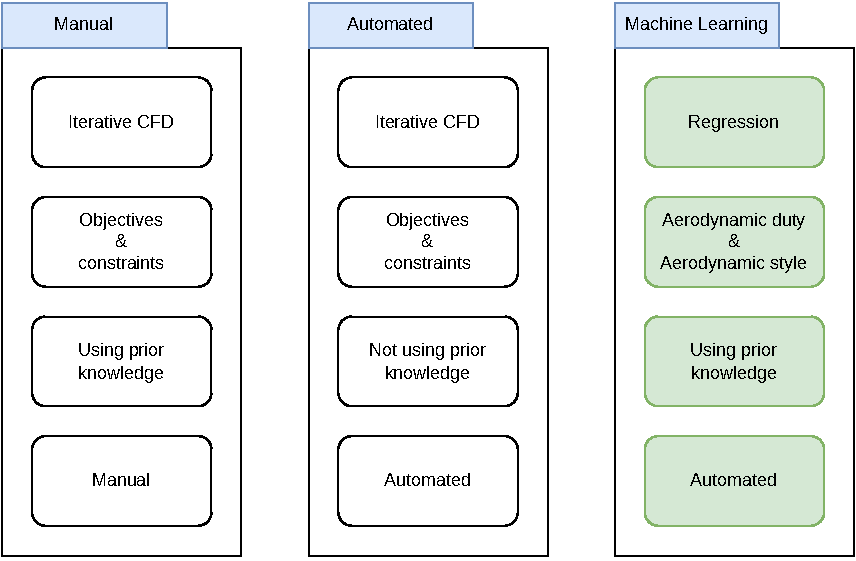
\includegraphics[page=1, scale=0.75]{pdf/designModes-04}
    \end{figure}
\end{frame}